0\let\negmedspace\undefined
\let\negthickspace\undefined
\documentclass[journal]{IEEEtran}
\usepackage[a5paper, margin=10mm, onecolumn]{geometry}
%\usepackage{lmodern} % Ensure lmodern is loaded for pdflatex
\usepackage{tfrupee} % Include tfrupee package

\setlength{\headheight}{1cm} % Set the height of the header box
\setlength{\headsep}{0mm}     % Set the distance between the header box and the top of the text

\usepackage{gvv-book}
\usepackage{gvv}
\usepackage{cite}
\usepackage{amsmath,amssymb,amsfonts,amsthm}
\usepackage{algorithmic}
\usepackage{graphicx}
\usepackage{textcomp}
\usepackage{xcolor}
\usepackage{txfonts}
\usepackage{listings}
\usepackage{enumitem}
\usepackage{mathtools}
\usepackage{gensymb}
\usepackage{comment}
\usepackage[breaklinks=true]{hyperref}
\usepackage{tkz-euclide} 
\usepackage{listings}
% \usepackage{gvv}                                        
\def\inputGnumericTable{}                                 
\usepackage[latin1]{inputenc}                                
\usepackage{color}                                            
\usepackage{array}                                            
\usepackage{longtable}                                       
\usepackage{calc}                                             
\usepackage{multirow}                                         
\usepackage{hhline}                                           
\usepackage{ifthen}                                           
\usepackage{lscape}
\begin{document}

\bibliographystyle{IEEEtran}
\vspace{3cm}

\title{NCERT 9.4.12}
\author{EE24BTECH11041 - Mohit}
% \maketitle
% \newpage
% \bigskip
{\let\newpage\relax\maketitle}

\renewcommand{\thefigure}{\theenumi}
\renewcommand{\thetable}{\theenumi}
\setlength{\intextsep}{10pt} % Space between text and floats
\begin{enumerate}
\item Solve the differential equation given below with initial conditions $ x = 2 $ and $ y = 0 $ and plot a graph.
\begin{align}
	x(x^2-1)\frac{dy}{dx}=1
\end{align}
\textbf{Solution:-}\\
\begin{enumerate}
    \item Rearranging the Equation,\\
    \begin{align}
	    dy = \frac{dx}{x(x^2-1)}
    \end{align}
    \item \textbf{Integration:} Integrating on both sides.\\   
    \begin{align}
    \int{dy} = \int{\frac{dx}{x(x^2-1)}} 
    \end{align}
    \begin{align}
    \int{dy} = \int{\frac{dx}{x^3(1-\frac{1}{x^2})}} 
    \end{align}
    \item Subsituting ,
    \begin{align}
    1-\frac{1}{x^2} = t
    \end{align}
    \item Differentiating on both side ,
    \begin{align}
    \frac{dx}{x^3}=\frac{dt}{2}
    \end{align}
    \item  Now integrating,
    \begin{align}
    \int{dy} = \int{\frac{dt}{2t}} 
    \end{align}
    \begin{align}
    y = \frac{1}{2}\ln{t} + c
    \end{align}
    \item substituting t,
    \begin{align}
    y = \frac{1}{2}\brak{\ln{\brak{1-\frac{1}{x^2}}}} + c
    \end{align} 
    \item finding constant by putting x=2 and y=0
    \begin{align}
    c = \frac{1}{2}ln{\frac{4}{3}}
    \end{align} 
    \item This leads to:
    \begin{align}
    y = \frac{1}{2}\brak{\ln{\frac{4}{3}\brak{1-\frac{1}{x^2}}}}
    \end{align}
    \item \textbf{NOTE:-} We are not using finite difference because the graph is discontinues at x=1 .So, when we find $\frac{dy}{dx}$ its value is becoming too large that we are getting a significant error in calculating $\frac{dy}{dx}$.So,We have to use another method.
    \item \textbf{CODING LOGIC:} The solution for the differential equation can be graphically solved using coding by using below logic :\textbf{Runga-kutta Method}
\begin{align} 
	h&=0.001 \\
\end{align}
\item Let ,
\begin{align} 
	\frac{dy}{dx} = f\brak{x_n} \\
	k_1 = hf\brak{x_n}\\
	k_2 = hf\brak{x_n + h/2}\\
	k_3 = hf\brak{x_n + h/2}\\
	k_4 = hf\brak{x_n + h}\\
	k = \frac{1}{6}\brak{k_1 + 2k_2 + 2k_3+k_4}\\
	y_{n+1} = y_n + k
\end{align}
\end{enumerate}

\end{enumerate}

\begin{figure}[h!]
   \centering
   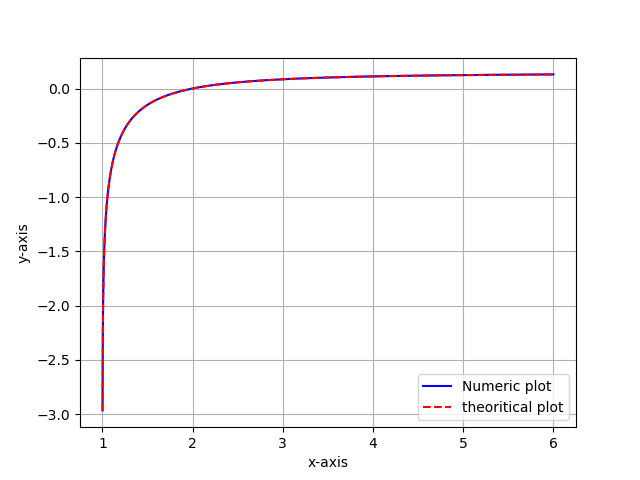
\includegraphics[width=0.7\linewidth]{figs/Figure_1.png}
   \caption{Plot of functions}
\end{figure}

\end{document}
